\chapter{硬件模块介绍}

\section{基于FIFO的可变长移位寄存器设计}

\begin{figure}[h]
    \centering
    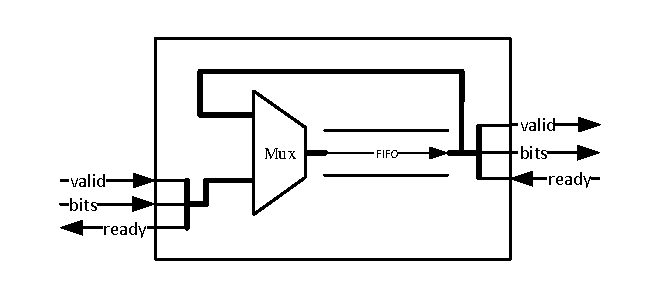
\includegraphics{../pdf/fifoshift.pdf}\\
    \caption{FIFO Shift}
\end{figure}
利用FIFO的先入先出特性,配合外部控制信号可以构造一个最大位宽为FIFO深度的移位寄存器。
首先,模块中的Mux将FIFO接口入模块输入信号连接,此时数据被写入FIFO中,当数据输入过程完成之后,Mux将模块内的FIFO输入与输出对接,
此时便形成了一个数据环路,FIFO输出的数据被输入给FIFO的输入,使数据一直保留在FIFO中。

实际使用时,FIFO深度被配置为256,位宽为16bit。第一阶段,FIFO输入通过Mux与模块的输入对接,接受来自外部的图像或者卷积核信息,第一阶段取数完成后进入第二阶段——计算,此时FIFO的输入与FIFO的输出对接,吐出的数据再次被存入FIFO中,以达到移位寄存器的功能。

需要说明的是,由于FIFO先入先出的特性,该移位构造,读数时每次只能读取最末端的数据,但相比与传统通过寄存器的构造,降低了资源占用率。

    \subsection{BRAM与DRAM选择}
    在Xilinx 7系FPGA中,片上RAM分为BRAM和DRAM两种,其中BRAM为板载RAM,是专门用于实现大容量RAM的部分,而DRAM是通过LUT构造的RAM。实际使用时,大容量RAM通常使用BRAM,但BRAM使用较为笨重,因为其是FPGA中的位置固定,会造成连线传输延时高的问题,同时BRAM时序比较严格,必须使用同步写入、同步读取的方式进行操作。而DRAM相对灵活,由于采用LUT构造,其能出现在FPGA绝大部分位置来最小化传输延时,同时DRAM可以进行异步读取操作,也可以在其后添加寄存器实现同步读取操作。本文所阐述的方案由于需要RAM具有异步读取操作,同时RAM容量小,数量多,因此采用DRAM。

\section{SRAM部分在FPGA中的优化}
Chisel3中构造存储器有两种方式,第一种通过VecInit构造ROM,FPGA实现时是通过线网。第二种通过MEM构造RAM,FPGA实现时是通过寄存器组。本文在设计过程中,首先通过MEM来构造片上RAM,但由于Chisel3 MEM自身的复杂度(其包含了Mask等附加功能),在实现一个6×7的PE阵列时,生成的代码量达到了16万行,通过Vivado综合一次需要90分钟,给调试工作带来了极大的不便利性,同时采用寄存器组的实现方式十分消耗资源。

由于ASIC中RAM通常需要特殊对待,本文在实际开发时,采用了Designware中的xxx ip核。优化之后生成的代码量下降至4万行,Vivado综合实现时间下降至5分钟。同时Designware中提供了ip的仿真模型,可以通过Verilator仿真器进行准确的仿真。

% \section{基于Xilixn 7Series FPGA片上DSP的高性能乘法器}

\section{PE单元构造}

\section{用于数据分发的简易NoC设计}

\section{PE阵列生成器}
    \subsection{计算流程}

\section{顶层接口设计}

\section{本章小结}
% \subsection{二级节标题}

% \subsubsection{三级节标题}

% \paragraph{四级节标题}

% \subparagraph{五级节标题}

% \section{脚注}

% Lorem ipsum dolor sit amet, consectetur adipiscing elit, sed do eiusmod tempor
% incididunt ut labore et dolore magna aliqua. Ut enim ad minim veniam, quis
% nostrud exercitation ullamco laboris nisi ut aliquip ex ea commodo consequat.
% Duis aute irure dolor in reprehenderit in voluptate velit esse cillum dolore eu
% fugiat nulla pariatur. Excepteur sint occaecat cupidatat non proident, sunt in
% culpa qui officia deserunt mollit anim id est laborum.
% \footnote{This is a long long long long long long long long long long long long
% long long long long long long long long long long footnote.}
